\graphicspath{{main/implementation/graphics}}

\section{Implementation}

% In this section you will describe what you did, and why you made the important decisions affecting your actions.  It's not a diary - don't write a blow-by-blow account of every little thing that happened.  Be selective and report those choices and techniques which made a difference.  Make sure you discuss what options you considered.  Explain how the criteria and methodology you used to select amongst different options (which tools are most appropriate, for example).

% It may help to imagine that you are reading this project in the future, trying to replicate the work without making the same mistakes along the way.  What would you need to know to make your job easier, and what is unimportant or obvious?  Explain how you implemented the design in the previous chapter.

% This is the place in which you would explain any novel or especially complex algorithms, data structures or systems you have used.

% Make it clear what you have done, and what is pre-existing.  For example, if you are using third party software libraries, describe how you have used them, and how they have benefited your project rather than simply what they do.  If you have built on a framework, make it clear how you have developed new functionality.

Simplest part of the development lifecycle.

\subsection{Development Utilities}

Software Quality
Github Jira Agile

How this brings code down from github.

Rust, added a layer onto the yocto to deploy application software on target

\begin{figure}[ht]
    \centering
    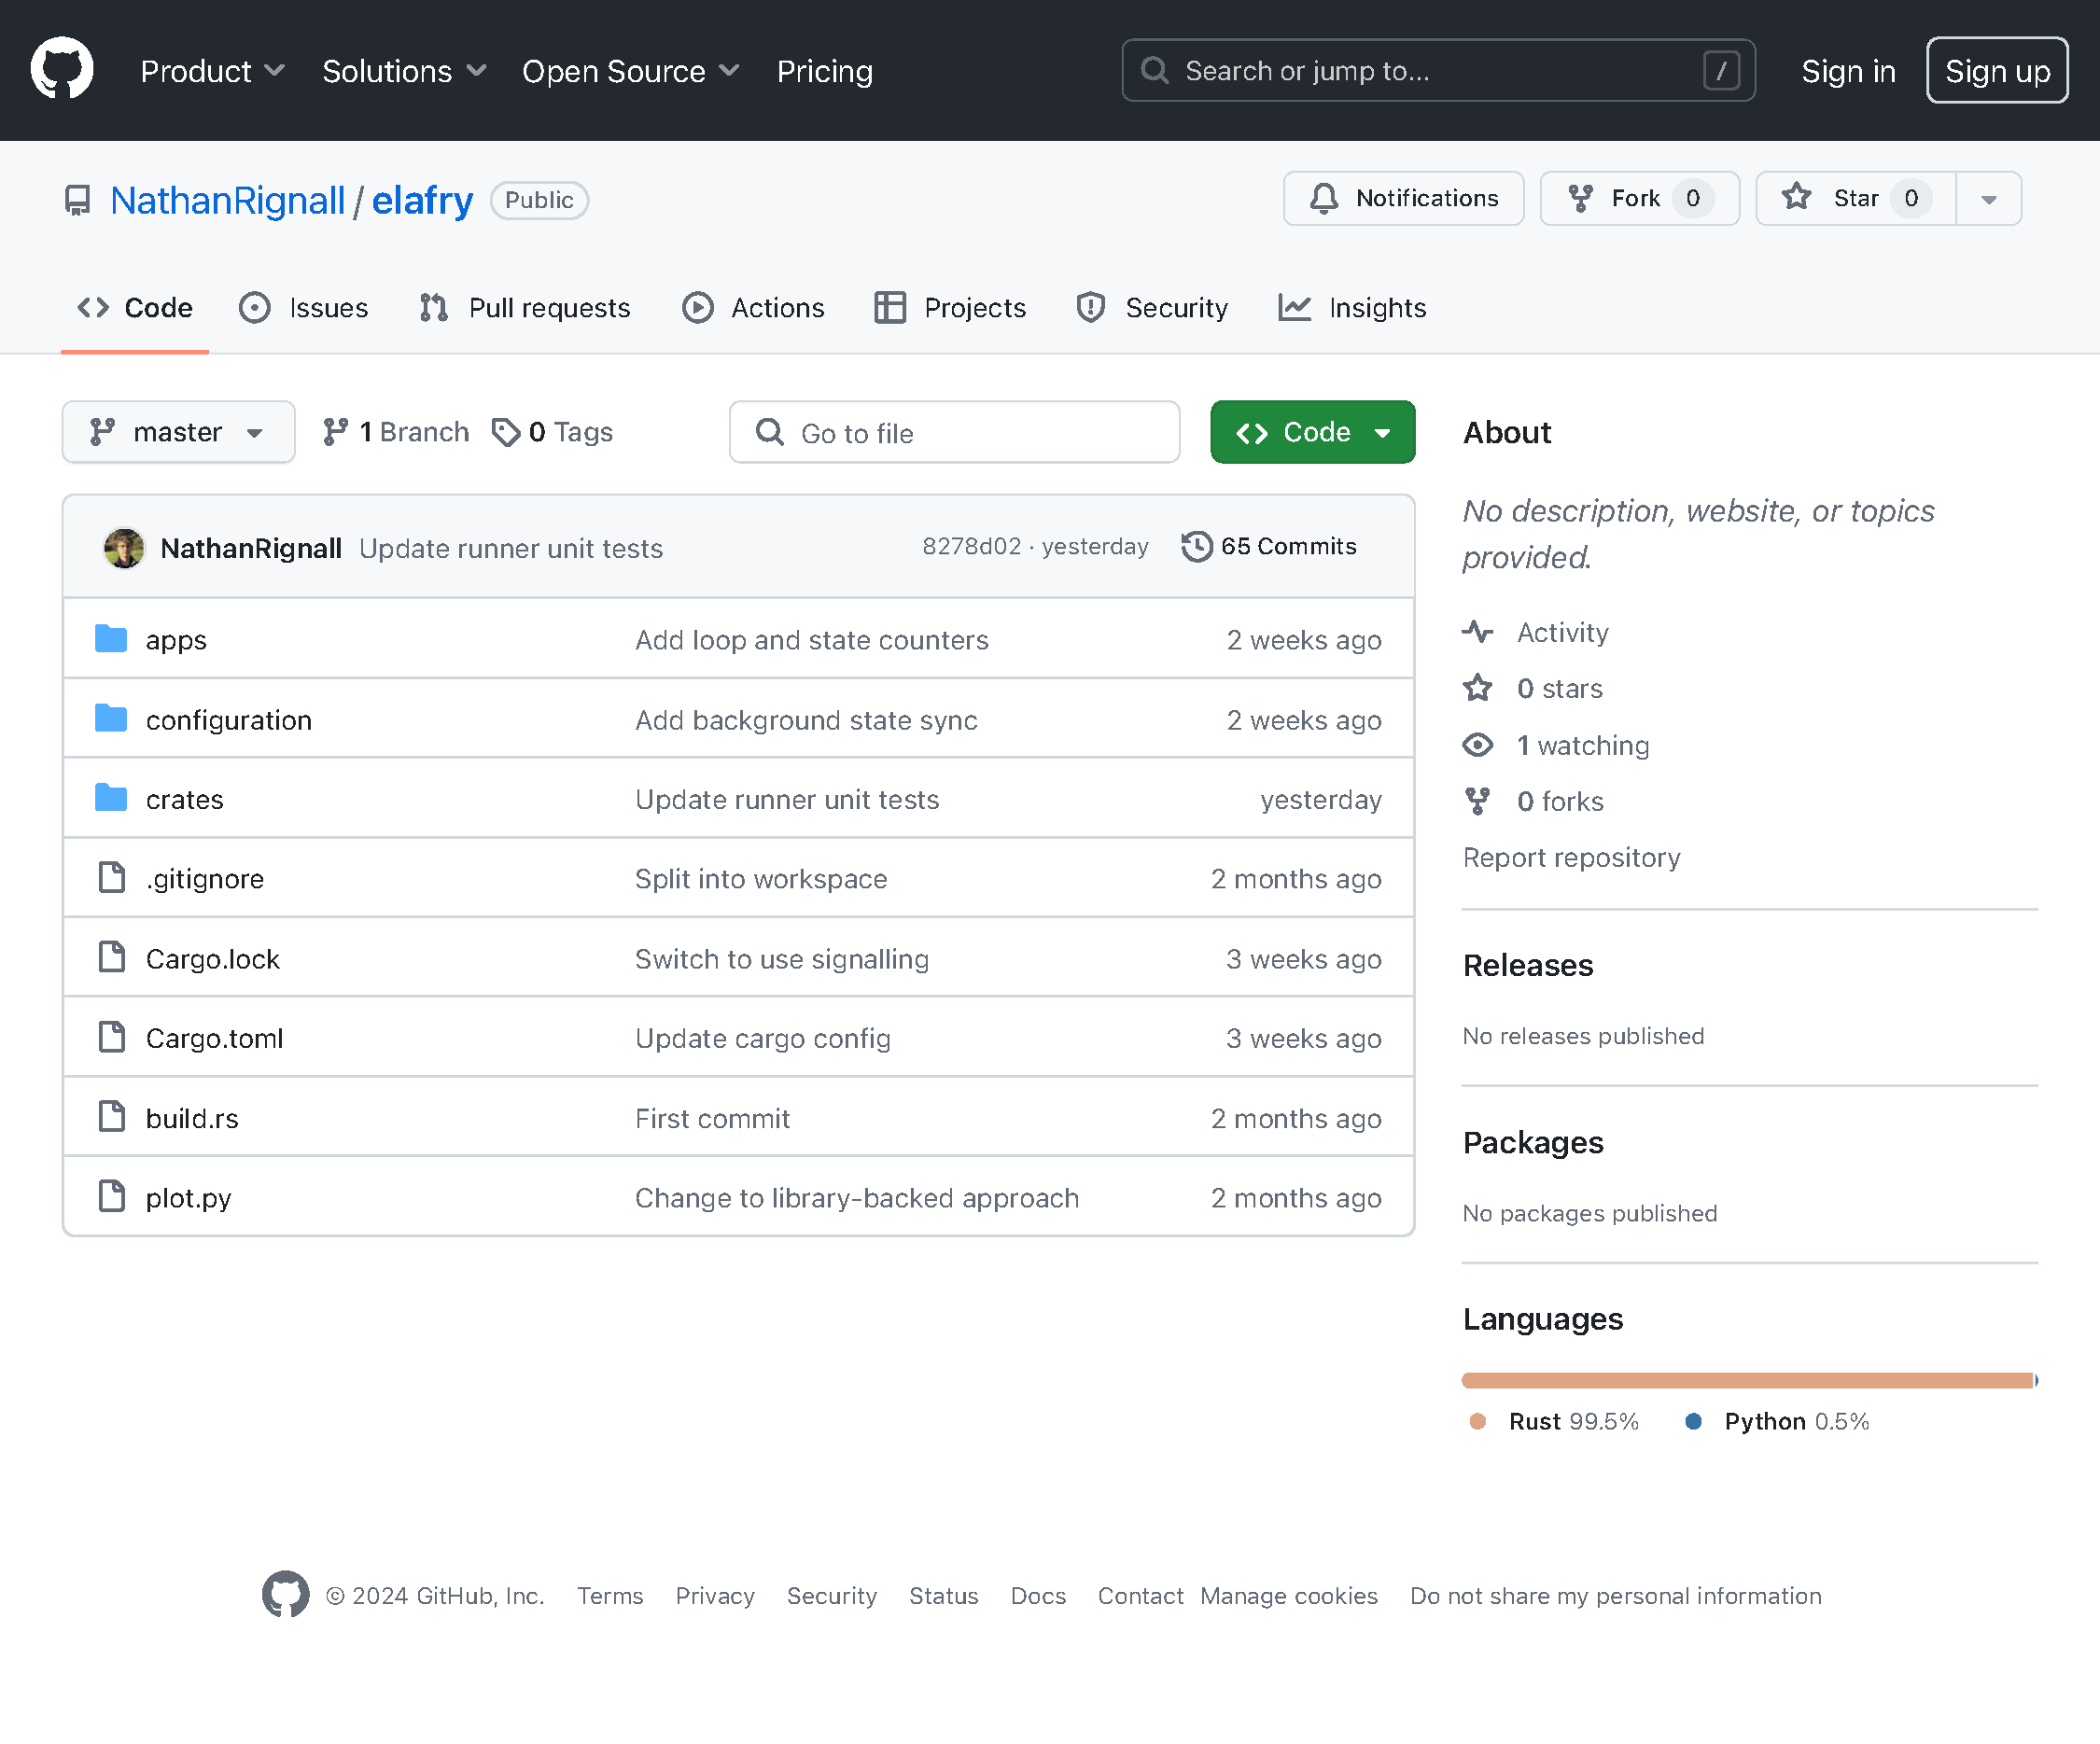
\includegraphics[width=\textwidth, clip, trim=0.1cm 5.2cm 0.1cm 2.6cm]{github.pdf}
    \caption[Github]
    {Github}
    \label{fig:implementationGithub}
\end{figure}

\subsubsection{Proessing Environment}
Did do some experimenting with unikernels and containers for the isolated processing environments
Picked processes in linux, theoriecally can add permisions with cgroups


\subsection{Software infrastructure}

Took the analysis of signals, applied this to implement the scheduler in Linux.

What libraries

Serde for data (yaml + bincode)
simple\_logger
uuid

With INFO, WARN, ERROR enabled.

divided into apps and crates

How do the classes fit together

Separate core library with management

structure of code


\subsubsection{Configurations}
Why YAML
YAML, and how they fit into a task list
Example YAML configuration


\subsection{Test Harness}

The intention for this software was to also use Rust, however could not get the Rust libaries for the W5500 working quickly, sure with extra time with sould have been possible.
To simplify this software the arduino development environment was used. This as all the drivers for the w5500 are integrated in arduino libraries.
